\section{Desarrollo} \label{desarrollo}
\AddToShipoutPictureBG*{
\includegraphics[width=\paperwidth,height=\paperheight]{Imagenes/Fondo Capitulo 2.pdf}}
\thispagestyle{plain}

\vspace{0.5cm}

\Large\scshape
\begin{center}
    {\Medium Diseño e implementación de la placa de circuito \\impreso de la plataforma de evaulación}
\end{center}
\normalfont
%\normalsize\vspace{2cm}

\divider

En este capítulo vamos a tratar la implementación de la plataforma experimental completa de la figura \ref{fig:plataforma_det} sobre una placa de circuito impreso. Dada la complejidad de todos los circuitos de este sistema, con una cantidad de componentes que supera los 150, se decidió  implementar una PCB doble faz o doble capa, con unas dimensiones de aproximadamene \SI[]{15}[]{\centi\metre} x \SI[]{15}[]{\centi\metre}. En tanto a su construcción, se utiliza el sustrato FR-4 estándar (laminado de resina epoxi reforzado con vidrio) y vías de tipo PTH (del inglés \textit{Plated Through-Hole}).\\

\begin{figure}[h]
    \centering
    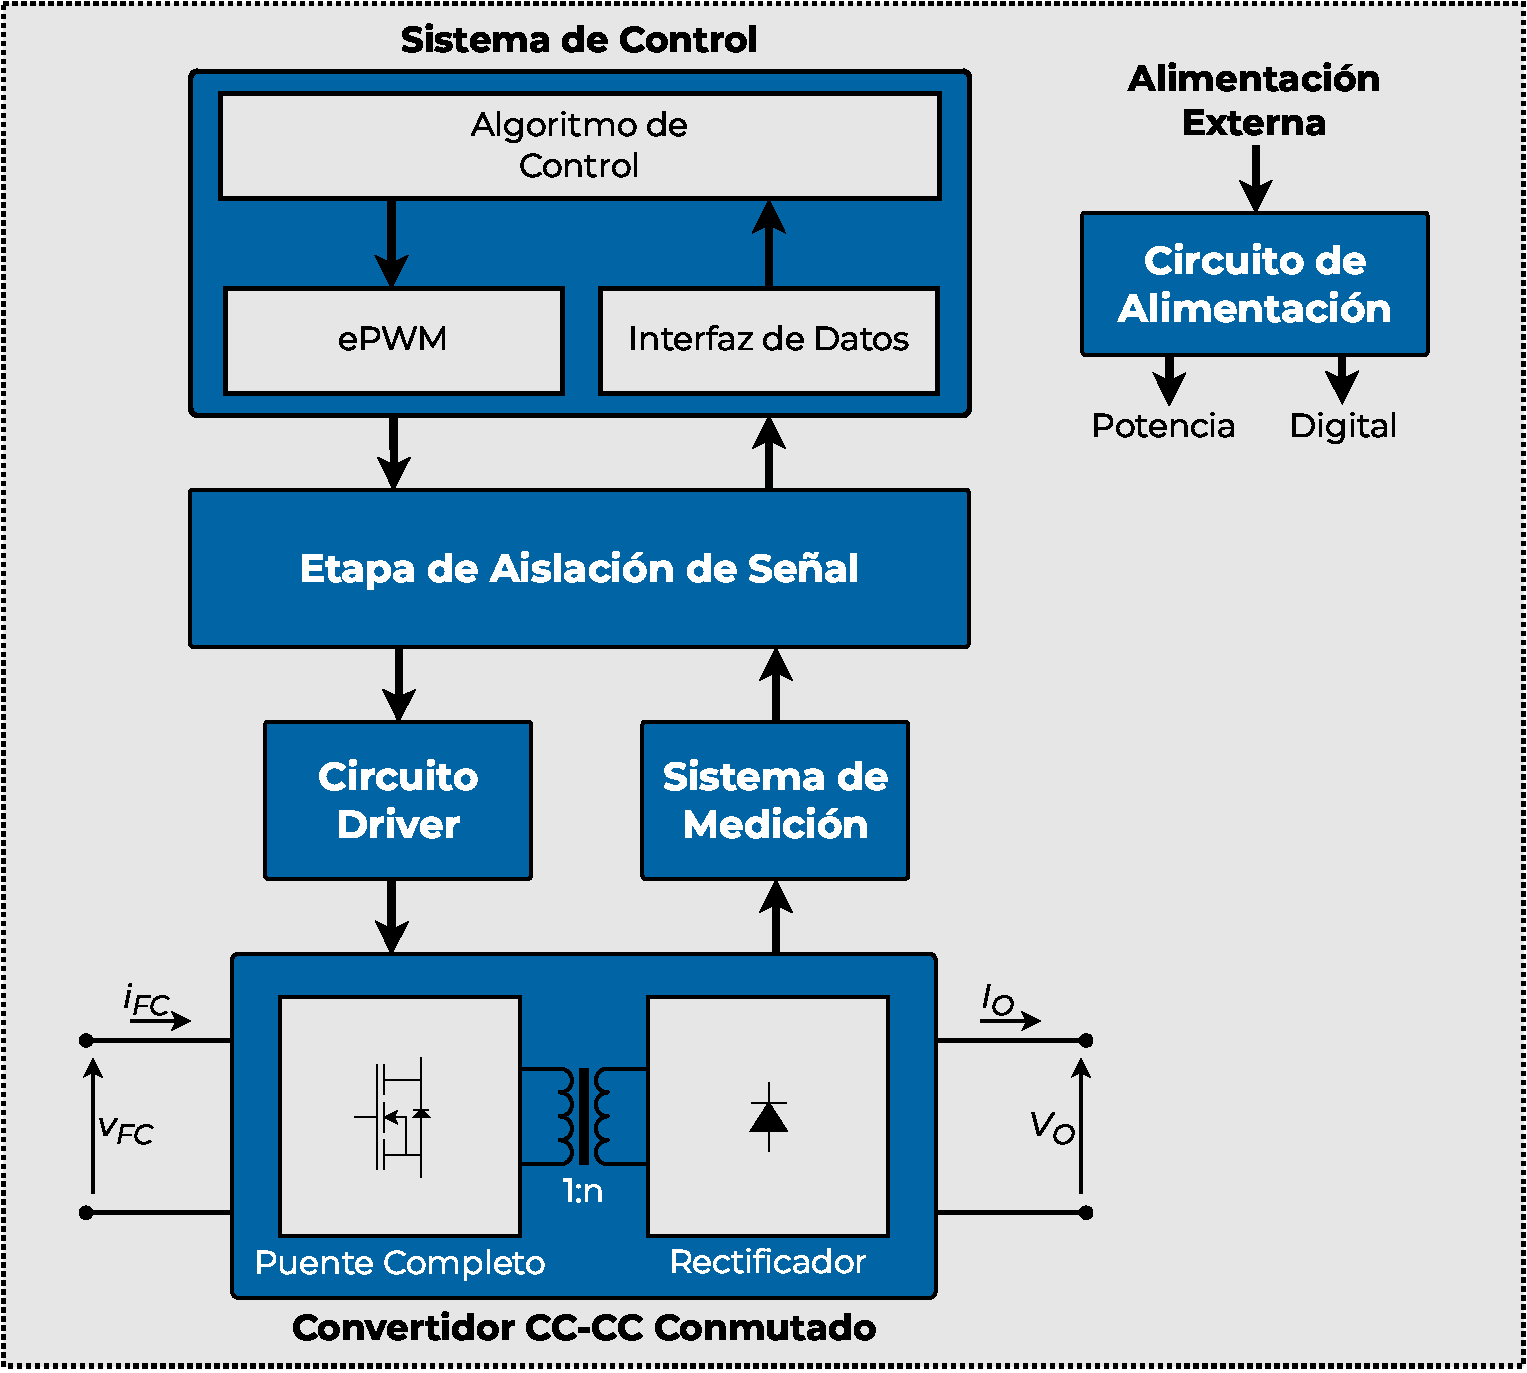
\includegraphics[scale=0.4]{Imagenes/Plataforma Detallada.pdf}
    \caption{Diagrama detallado de la plataforma experimental de evaluación, con los seis bloques que la componen.}
    \label{fig:plataforma_det}
\end{figure}

Como se ve en el diagrama detallado de la plataforma, esta cuenta con seis bloques principales a ser implementados en la plaqueta: los dos bloques principales (el convertidor y el bloque de control) y los cuatro bloques auxiliares restantes que se encargan de diversas tareas como la adquisición de datos y la alimentación de los circuitos, entre otras. Vamos a comenzar por una breve descripción de los circuitos de cada bloque y sus componentes, para luego pasar a la implementación de todos estos en la PCB, tomando en cuenta algunas consideraciones generales de diseño de PCB que vamos a establecer.\\

\subsection{Descripción Circuital}

\subsubsection{Convertidor CC-CC Conmutado}

En la figura \ref{fig:fullbridge} se presenta el circuito completo del convertidor CC-CC conmutado y aislado de tipo puente completo que se utiliza en la plataforma. Consiste de un puente de llaves con diodos en antiparalelo a cada una (de $Q_1$ a $Q_4$). Luego se encuentra un transformador de alta frecuencia que aisla los lados primario y secundario. El puente de diodos del secundario se encarga de generar una forma de onda rectificada, que es luego filtrada por el circuito LC y llevada en forma de corriente continua a la carga $R_L$.\\

\begin{figure}[h]
    \centering
    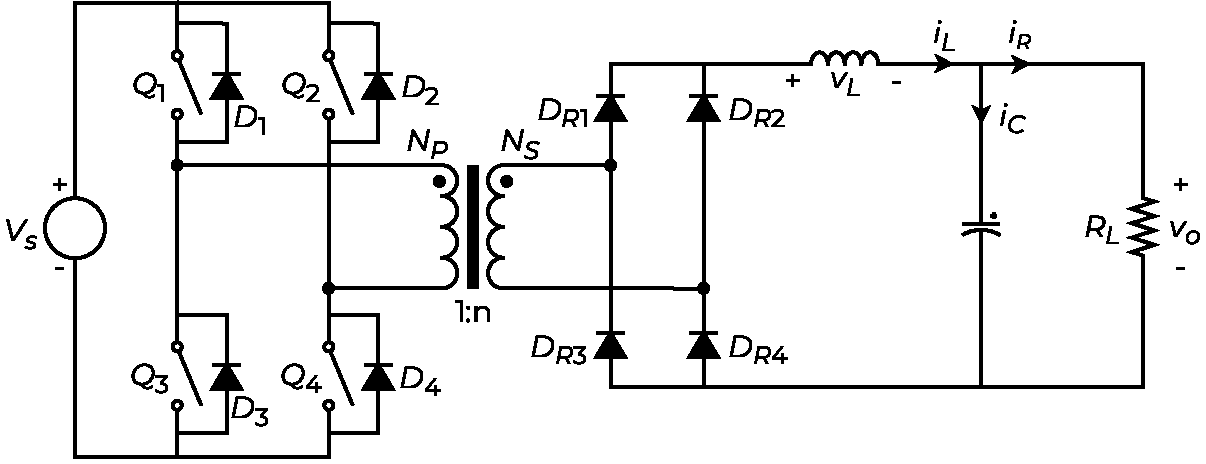
\includegraphics[scale=0.6]{Imagenes/Full Bridge.pdf}
    \caption{Diagrama del convertidor CC-CC de tipo puente completo a utilizar, con todos sus componentes.}
    \label{fig:fullbridge}
\end{figure}

Las funcionalidad de las llaves del primario es llevada a cabo por transistores MOSFET de potencia, cuyo modelo específico se trata más adelante. El lado primario y secundario se conectan a masas distintas ($GND_1$ y $GND_2$ respectivamente), ambas en el lado de potencia de la plataforma.\\

\subsubsection{Circuito Driver}

El circuito driver de la plataforma es el encargado de proveer los pulsos de tensión y corriente necesarios para excitar los MOSFET del puente de transistores y conmutarlos adecuadamente. Esta excitación es comandada por el sistema de control e ingresa por el tercer terminal de cada transistor, en este caso el \textit{gate}. Se observa el cricuito driver para una rama de transistores en la figura \ref{fig:driver}.\\

\begin{figure}[h]
    \centering
    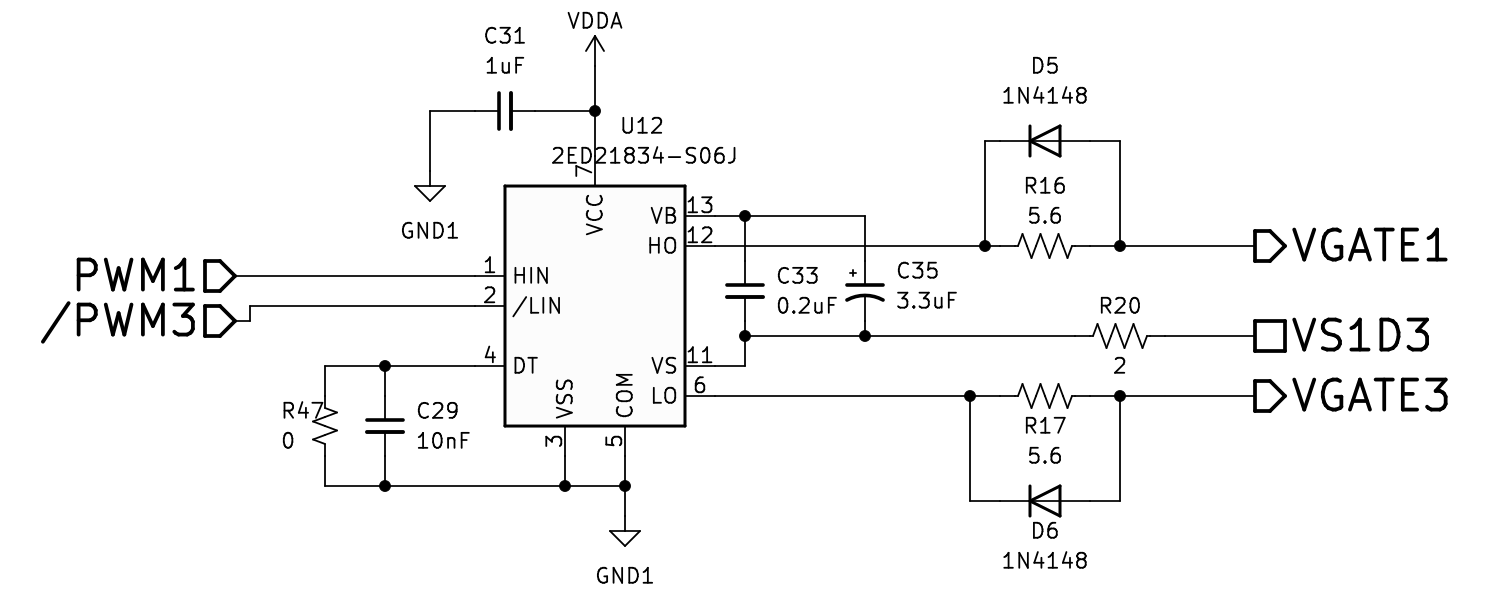
\includegraphics[scale=0.95]{Imagenes/Circuito Driver.png}
    \caption{Circuito de conexión del driver 2ED21834-S06J. El circuito del driver para la otra columna es idéntico.}
    \label{fig:driver}
\end{figure}

Si bien es posible diseñar un sistema de excitación con componentes discretos, resulta más sencillo y confiable utilizar componentes integrados que se encargan de realizar esta función, como el componente U12 que se observa en la figura (los componentes discretos que lo rodean están posicionados y dimensionados según recomendación del fabricante). Al estar encargado de la excitación de los transistores del primario, este circuito se encuentra puesto a tierra mediante la tierra primaria de potencia $GND_1$. Además, como el circuito de arriba es únicamente para una rama, se utiliza otro circuito idéntico para la rama restante de transistores.\\

\subsubsection{Sistema de Medición}

\lipsum[3]\\

\subsubsection{Etapa de Aislación de Señal}

\lipsum[4]\\

\subsubsection{Sistema de Control}

\lipsum[5]\\

\subsubsection{Circuito de Alimentación}

\lipsum[6]\\

\newpage

\subsection{Consideraciones Generales}

\subsubsection{Software EDA}

Para realizar el diseño de todos los esquemas circuitales del sistema, y luego plasmarlos a una placa de circuito impreso se debe utilizar un herramienta de automatización de diseño electrónico o EDA (del inglés \textit{Electronic Design Automation}). Existe una gran variedad de programas que cumplen este propósito, estando entre los más conocidos el \textit{Altium Designer} de \textit{Altium}, el \textit{EAGLE} de \textit{Autodesk}, el \textit{KiCad} y el \textit{Proteus Design Suite} de \textit{Labcenter Electronics}.\\

Para este proyecto se eligió utilizar la plataforma {\Medium KiCad} (que se encuentra en la versión 6.0.7 al momento de escribir este informe), una suite de software libre, gratuita y de código abierto que incluye todas la funcionalidades necesarias para el diseño electrónico. Cuenta con herramientas de captura de esquemático, diseño de PCB, simulación mediante SPICE o Ngspice, visualización de archivos de fabricación y cálculos de diseño de PCB.\\

\begin{figure}[h]
    \centering
    
\includegraphics[scale=0.6]{Imagenes/KiCad.pdf}
    \caption{Logotipo de la plataforma KiCad EDA.}
    \label{logo_kicad}
\end{figure}

El programa también cuenta con una extensa biblioteca de componentes y \textit{footprints} (son las \quotes{huellas} de los componentes en en el circuito impreso) y la capacidad de crear o importar bilbiotecas. Además tiene la capacidad de generar archivos de fabricación, modelos tridimensionales de la PCB y una \textit{bill of materials} (lista de componentes).\\


\subsubsection{Aislación de Tierras}

En toda la plataforma se va a trabajar con tres puestas a tierra distintas y aisladas entre sí: GND\textsubscript{1} es la tierra del primario del convertidor, GND\textsubscript{2} es la tierra del secundario del convertidor, y GND\textsubscript{D} es la tierra de las partes de señal y digitales, como los sensores y el DSC.\\

Esto, si bien agrega una mayor complejidad al diseño, es ventajoso por múltiples razones. Primero, evita la generación de interferencia de modo común entre las tierras del convertidor (GND\textsubscript{1} y GND\textsubscript{2}) que manejan altas corrientes y por lo tanto son más ruidosas; y la tierra de señal $GND_D$ de más bajas corrientes que es más sensible al ruido. Además, dadas las altas corrientes del convertidor, esta separación permite la protección de los circuitos de señal ante picos de corriente y tensión inesperados en la parte de potencia.\\

\subsubsection{Selección de Componentes}

Para todos los componentes en los que sea posible, se eligieron encapsulados de tamaño reducido y de montaje superficial (SMD, del inglés \textit{Surface Mounted Devices}). Estos son encapsulados, que como su nombre indica, son montados sobre la superficie de la placa, sin necesidad de una perforación que la atraviese (como es el caso de la tecnología THT o \textit{through-hole}). Esto facilita el ruteo de las pistas de cobre, dado que si una pista pasa por la capa opuesta de un componente SMD, no es necesario esquivar los pines del mismo, que se encuentran únicamente de un lado de la PCB.\\

Para componentes sencillos como capacitores, resistencias, diodos y LEDs, se elige, siempre que sea posible, los de tipo SMD de dimensiones 1206, que corresponden a un empaquetado de \SI[]{3}[]{\milli\metre} x \SI[]{1.5}[]{\milli\metre}.\\

\subsubsection{Ancho de Pistas}

La selección de los anchos de las pistas de cobre de las distintas partes del circuito es un parámetro sumamente importante, y presenta una situación de compromiso entre la superficie ocupada por las pistas y su pérdida de potencia (y elevación de temperatura). Para realizar estos cálculos se utiliza la herramienta \textit{PCB Calculator} incluida en la suite de KiCad, que tiene la capacidad de realizar múltiples cálculos de utilidad en el diseño de PCBs, incluido el cáclulo de ancho de pista, basado en la ecuación definida por la norma IPC-2221.

\begin{equation}\label{eq:IPC2221}
    I = K\cdot (\Delta T)^{\num{0.44}}\cdot (\num{1550}\cdot W\cdot H)^{\num{0.725}}
\end{equation}

Donde $I$ es la corriente que circula por la pista en [\unit{\ampere}], $K$ es una constante definida por la norma de valor \num{0.048} para pistas externas, $\Delta T$ es la elevación de temperatura de pista en [\unit{\celsius}], y $W$ y $H$ son el ancho y grosor de la pista en [\unit{\milli\metre}].\\

En nuestro caso, vamos a tomar un {\Medium grosor \textit{H} fijo de 0,035 mm} para ambas capas de cobre, que es un valor estándar; y una {\Medium elevación de temperatura de pista máxima de 20 °C}. Con estos valores fijados, se calculará el ancho $W$ de cada pista de la plaqueta.\\

Para las pistas de señal ubicadas en la parte digital de la plataforma, se decidió utilizar como estándar un ancho de pista $W$ de \SI[]{0.25}[]{\milli\metre}, que dadas las bajas corrientes que estas manejan (rara vez por encima de \SI[]{100}[]{\milli\ampere}), su temperatura no llega a elevarse ni \SI[]{1}[]{\celsius} según la ecuación \ref{eq:IPC2221}. Además, este es un ancho muy reducido, cercano a los limites de fabricación de múltiples fabricantes de placas locales.\\

\newpage

\subsection{Implementación en PCB}

Una vez definidos todos los circuitos que componen a la plataforma, se llega a un total de {\Medium 197 componentes} discretos con decenas de empaquetados distintos, que deben todos ser posicionados en una placa de circuito impreso doble faz del menor tamaño posible. El resultado final de la plaqueta, con todos sus componentes (exceptuando los disipadores térmicos de los transistores y diodos de potencia) se observa en la figura \ref{fig:PCB_3D}.\\

\begin{figure}[h]
    \centering
    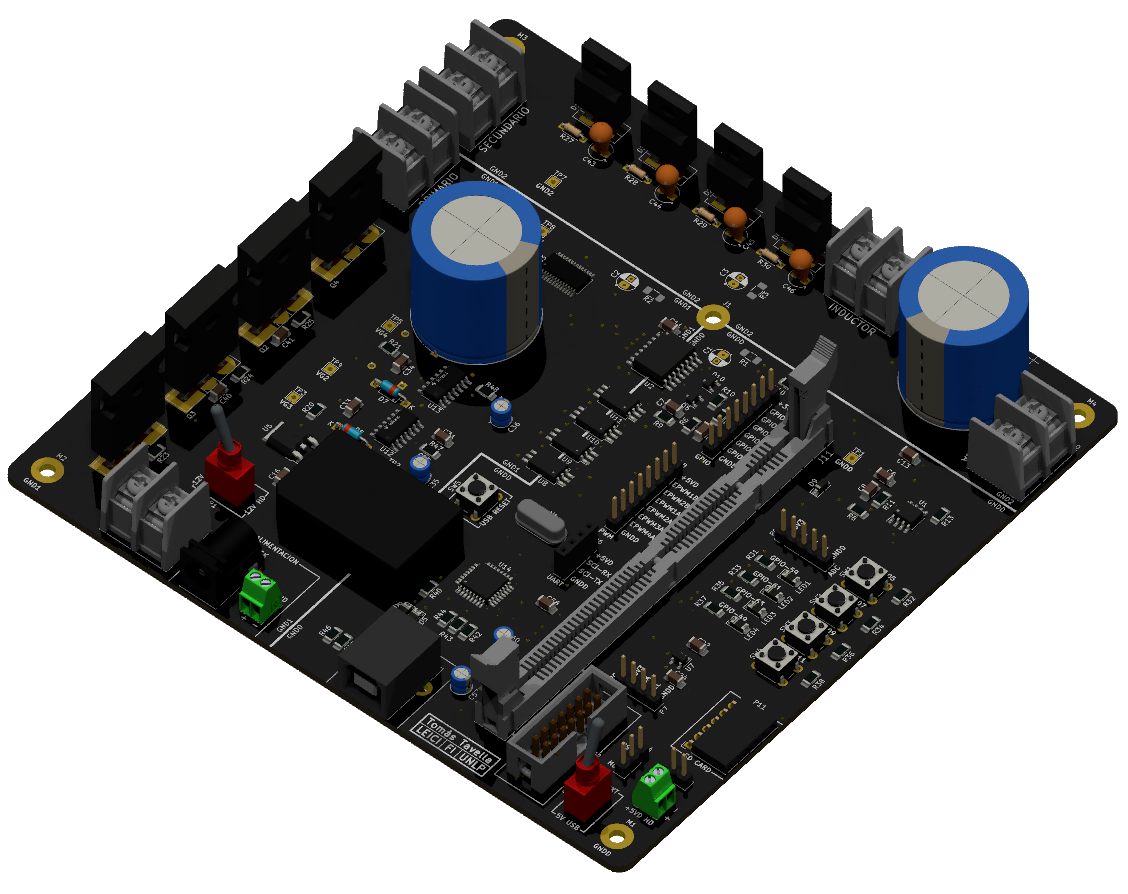
\includegraphics[scale=0.34]{Imagenes/PCB 3D Raytracing.png}
    \caption{Modelo tridimensional de la implementación en PCB de la plataforma con todos sus componentes, vista desde la parte superior.}
    \label{fig:PCB_3D}
\end{figure}

Para comenzar, se va a realizar un listado de todos los componentes, clasificados según sus distintos encapsulados y sus \textit{footprints} correspondientes (es la \quotes{huella} de cada componente sobre la plaqueta). Una vez establecido este listado, se procede a detallar el proceso de diseño de la placa de circuito impreso, comenzando por el posicionamiento de todos los componentes de la forma más compacta posible respetando la sepación de tierras y dando el espacio necesario para el ruteo de pistas. Finalmente se conectan todos los componentes según indica el esquema circuital de la plataforma, y se realizan verificaciones finales previo a la generación de los archivos de fabricación definitivos.\\

\subsubsection{Listado de Componentes}

En la tabla \ref{tabla:componentes} de la próxima página se presenta un listado de todos los componentes de la placa de circuito impreso, separados según su tipo de empaquetado, ya sea de montaje superficial (SMD) o de tipo through-hole (THT). Esto incluye circuitos integrados como los distintos sensores, resistencias y capacitores de todos los circuitos, transistores y diodos de potencia y auxiliares, y todos los distintos conectores de alimentación y señal.\\

\setlength{\tabcolsep}{8pt}
\renewcommand{\arraystretch}{1.45}
\begin{table}[H]
\begin{center}
    \begin{tabular}{llrl}
        & {\SemiBold Empaquetado} & {\SemiBold Cantidad} & {\SemiBold Descripción}\\
        \hline
        \multirow{14}{*}{\SemiBold SMD} & 1206 & \num{85} & Capacitores, Resistores y LED\\
        & 1210 & \num{1} & Capacitor Tantalio\\
        & 3 x 5.4 \unit{\milli\metre} & \num{2} & Capacitores Aluminio\\
        & 2512 & \num{1} & Resistor Shunt\\
        & SOIC-8 & \num{3} & Sensor Hall y otros\\
        & SOIC-16W & \num{1} & Aislador ISO7242C\\
        & HTSSOP-28 & \num{1} & Sensor LM5056A\\
        & SSO-6 & \num{4} & Optoacoplador ACPL-P480\\
        & SO-14 & \num{2} & Drivers 2ED21834-S06J\\
        & LQFP-32 & \num{1} & FTDI FT232BL\\
        & SOD-123 & \num{1} & Diodo Schottky\\
        & SOT-23 & \num{3} & Diodos Schottky y Transistores\\
        & SOT-23-5 & \num{2} & Reguladores Lineales\\
        & TO-252-2 & \num{1} & Regulador Lineal\\
        \hline
        \multirow{19}{*}{\SemiBold THT} & D25\unit{\milli\metre} & \num{2} & Capacitores Electrolíticos \SI[]{680}[]{\micro\farad}\\
        & D4\unit{\milli\metre} & \num{7} & Capacitores Electrolíticos\\
        & D4,5\unit{\milli\metre} & \num{4} & Capacitores Tantalio\\
        & D1,6\unit{\milli\metre} x L3,6\unit{\milli\metre} & \num{4} & Resistores\\
        & TO-247AC & \num{4} & Transistores IRFP150\\
        & TO-220 & \num{4} & Diodos MUR860\\
        & DIP-24 & \num{1} & Fuente Aislada THB3-1211\\
        & DO-35 & \num{4} & Diodos\\
        & HC-18 & \num{1} & Cristal\\
        & DIMM100 & \num{1} & Conector DIMM para DSC\\
        & DCJ200-10A & \num{1} & Barrel Jack\\
        & USB-B & \num{1} & Conector USB-B Hembra\\
        & Degson Screw Terminal & \num{5} & Conectores Pila, Carga, etc.\\
        & Phoenix Contact 2P & \num{2} & Conectores 5V y 12V Externo\\
        & Pulsador P6\unit{\milli\metre} & \num{5} & Pulsadores\\
        & Pin Header P2,54\unit{\milli\metre} & \num{34} & Tiras de Pines\\
        & Pin Header P2,54\unit{\milli\metre} 2x7 & \num{1} & Conector J-TAG\\
        & Pin Socket P2,54\unit{\milli\metre} & \num{6} & Conectores Pines Hembra\\
        & Switch 3P P2,54\unit{\milli\metre} & \num{2} & Interruptor de 3 Polos\\
        \hline
        {\SemiBold Total} & & {\SemiBold 197} &
    \end{tabular}
    \caption{Lista completa de componentes de la plataforma, clasificados según su tipo y modelo de encapsulado.}
    \label{tabla:componentes}
\end{center}
\end{table}

Ahora, todos estos componentes se deben posicionar de manera compacta en la placa doble faz de aproximadamente \SI[]{15}[]{\centi\metre} de lado, y conectarse de acuerdo a los circuitos presentados en la sección anterior, teniendo en cuenta las consideraciones de ancho de pista y conexión de tierras.\\

\subsubsection{Posicionamiento de Componentes}

Para comenzar la ubicación de los componentes en la plaqueta, primero debemos separar claramente todos los componentes en tres regiones distintas: los componentes que se conectan a la referencia digital GND\textsubscript{D}, los que se conectan a la referencia del primario GND\textsubscript{1}, y los que se conectan a la referencia del secundario GND\textsubscript{2}. Existe una pequeña selección de componentes, como por ejemplo el aislador ISO7242C, que se encuentran entre dos de estas zonas, por formar parte del circuito de aislación de señal de la plataforma.\\ 

\lipsum[4]\\

\newpage\afterpage{\blankpage}

\begin{figure}[H]
    \centering
    \subfigure[Capa de cobre frontal, con los distintos bloques de la plataforma indicados.]{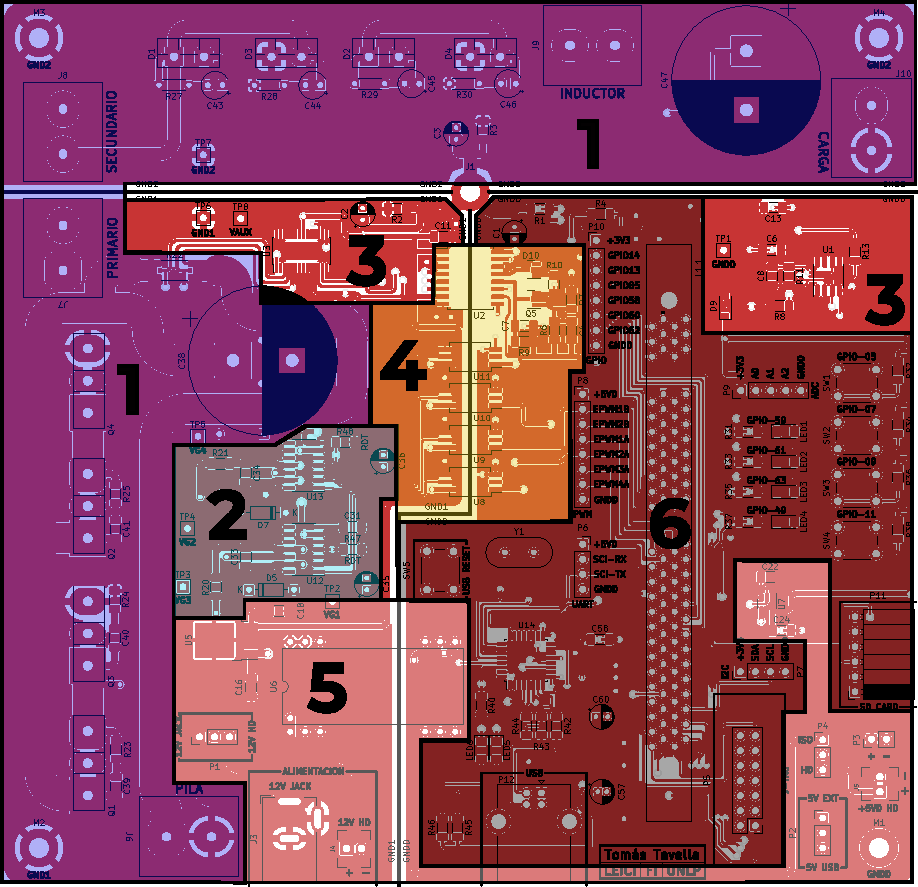
\includegraphics[scale=0.8]{Imagenes/PCB Front - SubCircuitos.pdf}}\\
    \subfigure[Capa de cobre trasera, con las tres distintas puestas a tierra.]{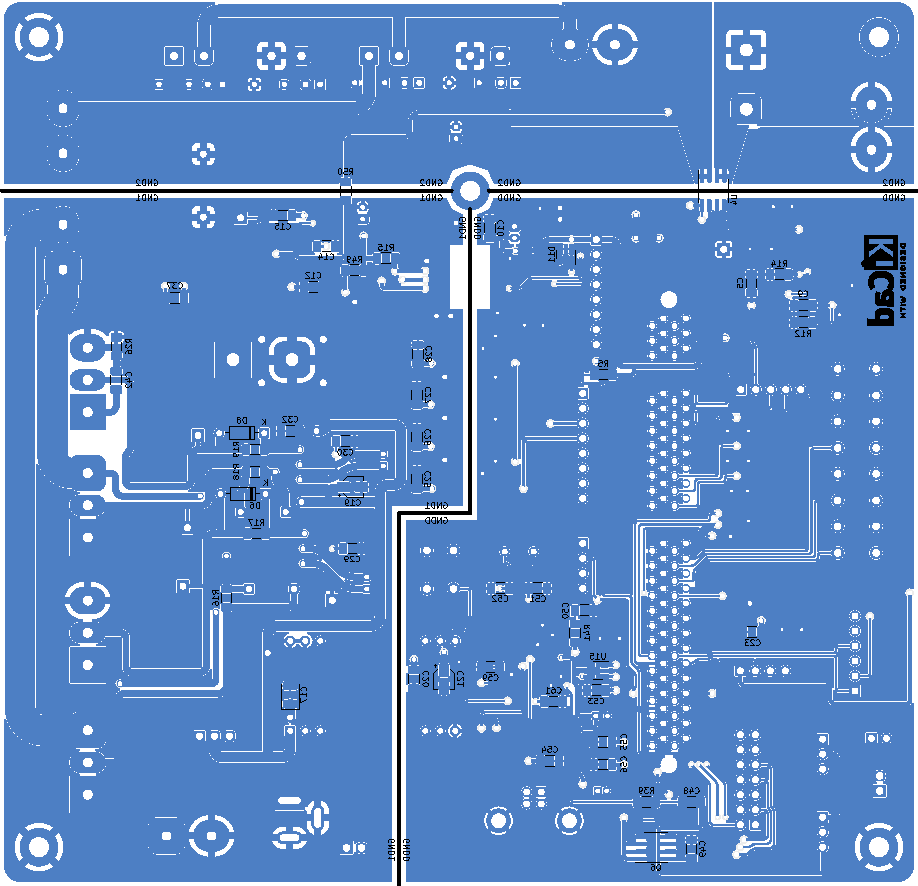
\includegraphics[scale=0.8]{Imagenes/PCB Back Layer.pdf}}%
    \caption{Diagrama de las distintas capas de cobre de la PCB.}
    \label{fig:PCB_cobre}
\end{figure}

\newpage